% Figure (new): the four MorphEvalHeb classifier configurations.
% Facts from the released checkpoints (huggingface.co/Amit5674/...) and models_finetune/*/training_args.txt.
% Compiles with pdfLaTeX, XeLaTeX or LuaLaTeX (no Hebrew). Natural width = 16cm (ACL \textwidth).
\documentclass[10pt,border=2pt]{standalone}
\usepackage{iftex}
\ifPDFTeX \usepackage{times} \else \usepackage{fontspec}\setmainfont{FreeSerif.otf}[BoldFont=FreeSerifBold.otf,ItalicFont=FreeSerifItalic.otf] \fi
\usepackage{amsmath}
\usepackage{tikz}
\usetikzlibrary{positioning,arrows.meta,fit,backgrounds,calc}
\definecolor{data}{HTML}{EFEFEF}   % inputs
\definecolor{enc}{HTML}{CFE3F3}    % NeoDictaBERT encoder
\definecolor{bin}{HTML}{D6EEDC}    % binary output
\definecolor{ml}{HTML}{FBE3C8}     % multi-label output
\begin{document}\hyphenpenalty=10000\exhyphenpenalty=10000
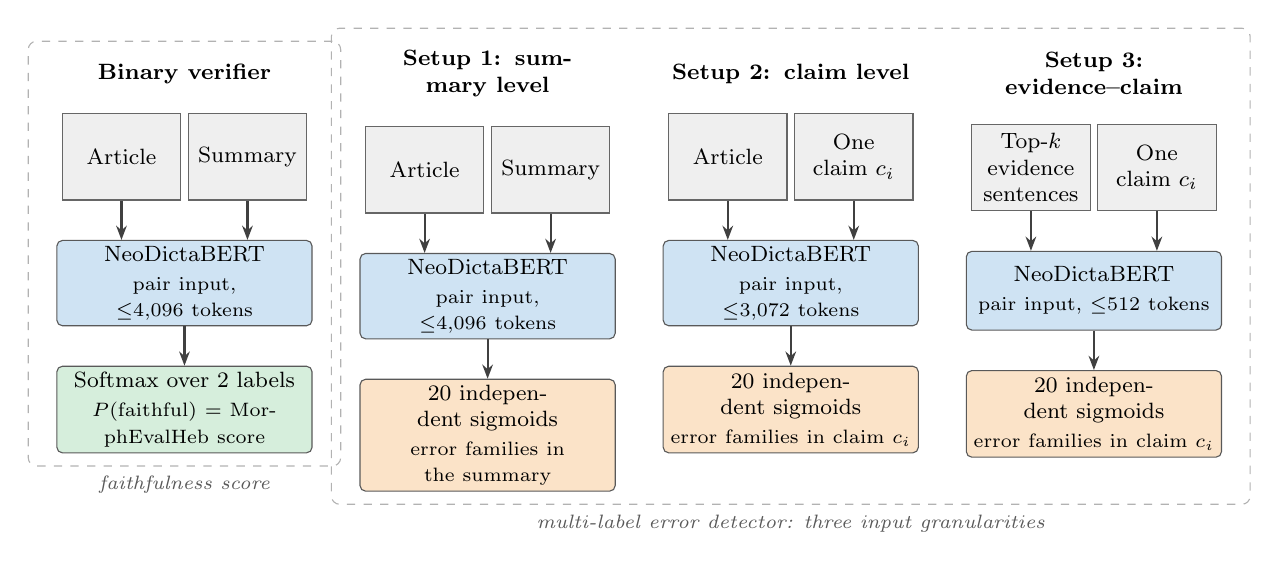
\begin{tikzpicture}[
  font=\footnotesize, >={Stealth[length=1.8mm]},
  inp/.style={draw=black!60, fill=data, align=center, text width=14mm, minimum height=11mm, inner sep=1.5pt, anchor=north},
  encb/.style={draw=black!65, fill=enc, rounded corners=2pt, align=center, text width=31mm, minimum height=10mm, inner sep=2pt},
  outb/.style={draw=black!65, rounded corners=2pt, align=center, text width=31mm, minimum height=11mm, inner sep=2pt},
  title/.style={font=\footnotesize\bfseries, align=center, text width=34mm},
  arr/.style={->, draw=black!75, thick},
  col/.style={draw=black!30, dashed, rounded corners=3pt, inner sep=1.6mm}]

% column x positions (cm)
\foreach \x/\n in {0/b, 3.85/s1, 7.7/s2, 11.55/s3} {
  \coordinate (\n) at (\x,0);
}

% ---------- titles ----------
\node[title] (tb)  at ($(b)+(0,0)$)  {Binary verifier};
\node[title] (t1)  at ($(s1)+(0,0)$) {Setup 1: summary level};
\node[title] (t2)  at ($(s2)+(0,0)$) {Setup 2: claim level};
\node[title] (t3)  at ($(s3)+(0,0)$) {Setup 3: evidence--claim};

% ---------- inputs ----------
\node[inp] at ($(tb.south)+(-8mm,-2.5mm)$)  (bA) {Article};
\node[inp] at ($(tb.south)+(8mm,-2.5mm)$) (bS) {Summary};
\node[inp] at ($(t1.south)+(-8mm,-2.5mm)$)  (1A) {Article};
\node[inp] at ($(t1.south)+(8mm,-2.5mm)$) (1S) {Summary};
\node[inp] at ($(t2.south)+(-8mm,-2.5mm)$)  (2A) {Article};
\node[inp] at ($(t2.south)+(8mm,-2.5mm)$) (2C) {One claim $c_i$};
\node[inp] at ($(t3.south)+(-8mm,-2.5mm)$)  (3E) {Top-$k$ evidence\\sentences};
\node[inp] at ($(t3.south)+(8mm,-2.5mm)$) (3C) {One claim $c_i$};

% ---------- encoder ----------
\node[encb, below=5mm of tb.south |- bA.south] (bE) {NeoDictaBERT\\[1pt]\scriptsize pair input, $\le$4{,}096 tokens};
\node[encb, below=5mm of t1.south |- 1A.south] (1E) {NeoDictaBERT\\[1pt]\scriptsize pair input, $\le$4{,}096 tokens};
\node[encb, below=5mm of t2.south |- 2A.south] (2E) {NeoDictaBERT\\[1pt]\scriptsize pair input, $\le$3{,}072 tokens};
\node[encb, below=5mm of t3.south |- 3E.south] (3E2) {NeoDictaBERT\\[1pt]\scriptsize pair input, $\le$512 tokens};

% ---------- heads / outputs ----------
\node[outb, fill=bin, below=5mm of bE] (bO) {Softmax over 2 labels\\[1pt]\scriptsize $P(\text{faithful})$ = MorphEvalHeb score};
\node[outb, fill=ml, below=5mm of 1E] (1O) {20 independent sigmoids\\[1pt]\scriptsize error families in the summary};
\node[outb, fill=ml, below=5mm of 2E] (2O) {20 independent sigmoids\\[1pt]\scriptsize error families in claim $c_i$};
\node[outb, fill=ml, below=5mm of 3E2] (3O) {20 independent sigmoids\\[1pt]\scriptsize error families in claim $c_i$};

% ---------- arrows ----------
\foreach \i/\e/\o in {bA/bE/bO, bS/bE/bO, 1A/1E/1O, 1S/1E/1O, 2A/2E/2O, 2C/2E/2O, 3E/3E2/3O, 3C/3E2/3O} \draw[arr] (\i) -- (\i |- \e.north);
\foreach \e/\o in {bE/bO, 1E/1O, 2E/2O, 3E2/3O} \draw[arr] (\e) -- (\o);

% ---------- columns + group labels ----------
\begin{scope}[on background layer]
  \node[col, fit=(tb)(bA)(bS)(bO)] (cb) {};
  \node[col, fit=(t1)(1A)(1S)(1O)(t3)(3E)(3C)(3O)] (cm) {};
\end{scope}
\node[font=\scriptsize\itshape, text=black!65, anchor=north] at (cb.south) {faithfulness score};
\node[font=\scriptsize\itshape, text=black!65, anchor=north] at (cm.south) {multi-label error detector: three input granularities};
\end{tikzpicture}
\end{document}
